\chapter{Aufgabe 3}

\section{Teil 1}

\textit{Erstellen Sie eine Wahrheitstabelle für eine Digitalschaltung, die das Paritätsbit (bei gerader Parität) berechnet.
Wir gehen im Folgenden davon aus, dass vier Bits übertragen werden sollen,  die durch eine Digitalschaltung mit einem Paritätsbit ergänzt werden sollen.} \\

\noindent
Beispiel für ein Wort (4 Bit, + 1 Paritätsbit), das, unter Angabe gerader Parität, als korrekt übertragen gilt:

\begin{equation}\notag
    \texttt{0 0 0 0 | 0}
\end{equation}

\noindent
Das zu übertragende Wort besteht aus $4$ Bit, die allesamt auf $0$ gesetzt sind.\\
Die Anzahl der $1$en in dem Wort ist \textit{gerade} (da $2|0$).\\
In dem Fall muss das Paritätsbit (bei \textit{gerader} Parität) ebenfalls auf $0$ gesetzt werden, denn

\begin{itemize}
    \itemsep0.5em
    \item wird statt der \texttt{0 0 0 0} bspw. \texttt{0 1 0 0} übertragen (Informationswort \texttt{0 1 0 0 | 0}), ist die Anzahl der übertragenen $1$en in dem Wort \textit{ungerade}, das Paritätsbit müsste demnach auf $1$ gesetzt sein, ist aber auf $0$ gesetzt
    \item ist das Wort \texttt{0 0 0 0} und das Paritätsbit $1$ (das Informationswort also \texttt{0 0 0 0 | 1}), gilt das Signal ebenfalls als fehlerhaft, da nun wieder eine ungerade Anzahl von $1$en übertragen wurde, das Paritätsbit aber eine gerade Anzahl an $1$en erwartet.
\end{itemize}

\noindent
Beispiel für ein Wort ($4$ Bit) mit ungerader Anzahl von $1$en, + Paritätsbit:

\begin{itemize}
    \itemsep0.5em
    \item \texttt{0 1 0 0 | 1}: korrekt, da insgesamt $2$ Bit auf $1$ gesetzt sind - inkl. Paritätsbit
    \item \texttt{0 1 0 1 | 1}: fehlerhaft, Paritätsbit gibt an, dass gerade Anzahl an $1$en erwartet wurde, es finden sich aber $3$ Bit in dem Informationswort, die jeweils auf $1$ gesetzt sind.
\end{itemize}

\noindent
Insgesamt ergibt sich damit Kombination der Eingangssignale mit dem jeweils berechneten Paritätsbit wie in Tabelle~\ref{tab:paritätsbit} angegeben.


\begin{table}[ht]
    \setlength{\tabcolsep}{0.5em}
    \def\arraystretch{1.5}
    \centering
   \begin{tabular}{|c|c|c|c|c||c|}
        \hline
        \textbf{Zeile} & $A_3$ & $A_2$ & $A_1$ & $A_0$ & $y$ \\
        \hline \hline
        0  & 0 & 0 & 0 & 0 & 0 \\ \hline
        1  & 0 & 0 & 0 & 1 & 1 \\ \hline
        2  & 0 & 0 & 1 & 0 & 1 \\ \hline
        3  & 0 & 0 & 1 & 1 & 0 \\ \hline
        4  & 0 & 1 & 0 & 0 & 1 \\ \hline
        5  & 0 & 1 & 0 & 1 & 0 \\ \hline
        6  & 0 & 1 & 1 & 0 & 0 \\ \hline
        7  & 0 & 1 & 1 & 1 & 1 \\ \hline
        8  & 1 & 0 & 0 & 0 & 1 \\ \hline
        9  & 1 & 0 & 0 & 1 & 0 \\ \hline
        10 & 1 & 0 & 1 & 0 & 0 \\ \hline
        11 & 1 & 0 & 1 & 1 & 1 \\ \hline
        12 & 1 & 1 & 0 & 0 & 0 \\ \hline
        13 & 1 & 1 & 0 & 1 & 1 \\ \hline
        14 & 1 & 1 & 1 & 0 & 1 \\ \hline
        15 & 1 & 1 & 1 & 1 & 0 \\
        \hline
    \end{tabular}
    \caption{Lösungsvorschlag für Aufgabe 3.1}
    \label{tab:paritätsbit}
\end{table}

\section{Teil 2}

\textit{Erstellen Sie das zugehörige KV-Diagramm.
Versuchen Sie, die Schaltfunktionen zu vereinfachen, indem Sie benachbarte Eins-Felder zu Blöcken zusammenzufassen. Markieren Sie diese Blöcke im KV-Diagramm.}\\

\noindent
Das KV-Diagramm ist in Abbildung~\ref{fig:kv_parität} angegeben.\\
Es zeigt sich, dass keine Blöcke zusammengefasst werden können.


\begin{figure}
    \centering
    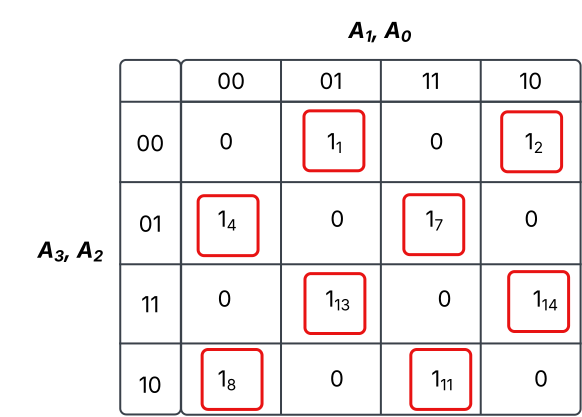
\includegraphics[scale=0.5]{aufgabe 3/img/kv_parität.svg}
    \caption{KV-Diagramm für Aufgabe 3.2. Tiefgestellte Ziffern beziehen sich auf die zugehörigen Zeilen in Tabelle~\ref{tab:paritätsbit}.  (Quelle: eigene)}
    \label{fig:kv_parität}
\end{figure}
